\section{Inter-simple sequence repeats (ISSRs)}

Inter-Simple Sequence Repeats (ISSRs) are sections of DNA located between microsatellites (=‘Simple Sequence Repeats’ (SSRs)) in an organism's genome \citep{Zietkiewicz1994, wolfe2005issr, Gaskin2011} (Fig. \ref{fig:issr}). Microsatellites are sequences of repeated DNA motifs that usually occur randomly at multiple loci in a genome, range from one to six nucleotides in length, and display a high mutation rate \citep{Gaskin2011, Hoy2013}. The ISSRs between these regions are particularly useful in detecting intraspecific variation due to their polymorphic nature \citep{Abbot2001}. In other words, each individual displays unique ISSR fragment sizes throughout their genome, which can be detected through the visualisation of banding patterns on an agarose gel and/or through capillary electrophoresis. ISSR primers typically consist of dinucleotide or trinucleotide base repeats \citep{wolfe2005issr}. ISSR analysis was developed in 1994, and was originally used to differentiate between plant cultivars \citep{wolfe2005issr}. Its application later extended to a wide range of other taxonomic groups, such as fungi \citep{kerrigan2003ascobotryozyma}, molluscs \citep{casu2005fine, casu2006inter}, birds \citep{haig2003parentage, wink2006use}, crocodiles \citep{machkour2009between}, snakes \citep{guicking2006introduced, nagy2007species}, lizards \citep{joger2007phylogeography}, tarantulas \citep{machkour2009issr}, sphingid moths (Lepidoptera: Sphingidae) \citep{hundsdoerfer2006incongruence}, the diamondback moth (\textit{Plutella xylostella} L.) \citep{roux2007issr}, lac insects (\textit{Kerria} spp.) \citep{saha2011genetic}, and silkworms (\textit{Bombyx mori} L.) \citep{chatterjee2003identification}. The technique has been used in the field of biological control in recent years, such as the genetic matching of invasive weeds to their native range \citep{paterson2013issrs, barker2015barcoding, Sutton2017GeneticAgents} and the detection of cryptic species \citep{Paterson2016} and genetic diversity \citep{Taylor2011GeneticMiridae} within the insect agent \textit{Eccritotarsus catarinensis} Carvalho (Hemiptera: Miridae), which is used for the biological control of water hyacinth. 
ISSR analysis is advantageous for the following reasons: \vspace{0.4cm}

\begin{enumerate}
    \item Primers are universal and can be used without prior knowledge of the target genomic sequence \citep{Wolfe1998, Gaskin2011}.
    \item ISSRs are abundant in the genomes of a wide variety of taxonomic groups and are highly informative and reproducible.
    \item The method is quick and cost-effective relative to other genotyping methods such as AFLP\textsuperscript{\textregistered} (amplified fragment length polymorphism) and RFLP (restriction fragment length polymorphism) \citep{Zietkiewicz1994, bornet2001nonanchored, bornet2004issr, DNAFragAnalysis}.
    \item The mutation rate of microsatellite regions is rapid \citep{wan2004genetic, DNAFragAnalysis}.
    \item Inherited microsatellite alleles are stable over multiple generations, and can be used at the population and individual level \citep{DNAFragAnalysis}.
\end{enumerate}

\subsection{Caveats of inter-simple sequence repeats}

\citet{meudt2007almost} state that AFLPs tend to outperform ISSRs and RAPDs (random amplified polymorphic DNA) in terms of lower genotyping error and higher robustness and informativeness. A number of studies involving crop cultivars and other plants have compared different fragment analysis methods, and many have supported this statement \citep{jones1997reproducibility, mcgregor2000comparative, hodkinson2002characterization, archak2003comparative, garcia2004comparison, behera2008relative, costa2016comparison}. \newline
Genotyping error refers to the differences between the genotypic data obtained independently from the same sample \citep{bonin2004track}.
The two overarching causes of such errors associated with `band-based' methods (including AFLPs and RAPDs) are allele homoplasy and scoring errors \citep{,bonin2004track, bonin2007statistical, holland2008optimizing}. 

\subsubsection{Homoplasy}
The term `homoplasy' means that the same characteristic has evolved independently in two or more otherwise different entities/species. Allele homoplasy thus refers to instances where fragments appear at the same position on a gel or an electropherogram, but are non-homologous \citep{bonin2007statistical, simmons2007penalty}. This phenomenon appears to increase in frequency in smaller fragments and in dense profiles, and when taxonomic distance increases; such that its effect on intraspecific comparisons is negligible \citep{bonin2007statistical}. Conversely, a particular locus may have undergone a mutation, insertion or deletion, resulting in the appearance of two or more independent loci that are actually linked \citep{simmons2007penalty}. \citet{simmons2007penalty} also mention the concerns around the origins of the amplified fragments (i.e. whether they are from the nuclear or mitochondrial genome, or whether they are in fact contaminants from hosts, parasites, or symbionts). 

\subsubsection{Error rates}
Data scoring is considered to be the main source of errors in fragment analysis procedures due to the high level of subjectivity involved at various stages of the analysis process \citep{bonin2004track}. Scoring errors for ISSRs can be largely overcome through the replication of each sample at the polymerase chain reaction (PCR) step. The most important determining factors in the comparison of replicate samples include:
\vspace{0.4cm}
\begin{enumerate}
    \item Differences in band intensity and what the peak height threshold is set at (i.e. what level of fluorescence is considered background noise, and how the number of false positive and negative calls can be minimised?).
    \item The bin width applied to score the presence and absence of bands (i.e. how strict or lenient should one be when determining whether a band occurs at the same locus in a replicate pair? What level of leeway should there be? If the bin width is too large, otherwise separate characters will be grouped as one, whereas a bin width that is too small will result in the scoring of numerous characters which are actually only representative of one locus) (Fig. \ref{fig:scoring_errors}). 
\end{enumerate}
\vspace{0.4cm}

\noindent Error rates are typically calculated as the average ratio between the number of mismatches and the total number of instances where a band was present, and absent, in both replicates (referred to as the Euclidean error rate) \citep{pompanon2005genotyping, bonin2007statistical}. It is suggested that an alternative error rate (the Jaccard error) should be calculated to complement the Euclidean error value. The Jaccard error calculation does not consider the shared absence of a band, as this absence may not be biologically meaningful \citep{holland2008optimizing}. AFLP Euclidean error rates typically range between 2 and 5\%, but \citet{bonin2007statistical} suggest that it should ideally not exceed 1\%. \citet{holland2008optimizing}, however, suggest that inter-study comparisons of error rates are not always reliable, as they encompass both PCR and scoring errors, and varying levels of divergence and data set size. Their study, for example, yielded AFLP error rates of 9 to 18\% and 6 to 13\% for sweet potato (\textit{Ipomoea batatas} (Convolvulaceae)) and \textit{Ourisia} (Plantaginaceae), respectively. Additionally, most of the studies reporting genotyping errors refer to AFLP techniques, and so it is unclear to what degree ISSR error rates are comparable. Surveys conducted by \citet{guichoux2011current} and \citet{bonin2004track} found that only between 6 and 26\% of papers, respectively, dealing with microsatellites reported error rates.  

\subsection{ISSRs as an identification tool}
Due to the significantly higher mutation rate in microsatellites compared to other DNA regions \citep{Zietkiewicz1994, Reddy2002}, ISSRs can offer higher resolution results that reveal greater differences between groups. This could be valuable in cases where traditional DNA barcoding regions are not sufficient in differentiating between closely related taxa, such as intraspecific lineages and different population groups. Fragment analysis methods, such as ISSRs, can therefore be used as molecular barcodes through the creation of unique fingerprint profiles (see for example \citet{galbacs2009identification}, \citet{adhikari2015efficiency}, \citet{li2018establishment}, and \citet{zhao2019molecular}).

\vspace{0.5cm}

\begin{figure}[H]
	\centering
	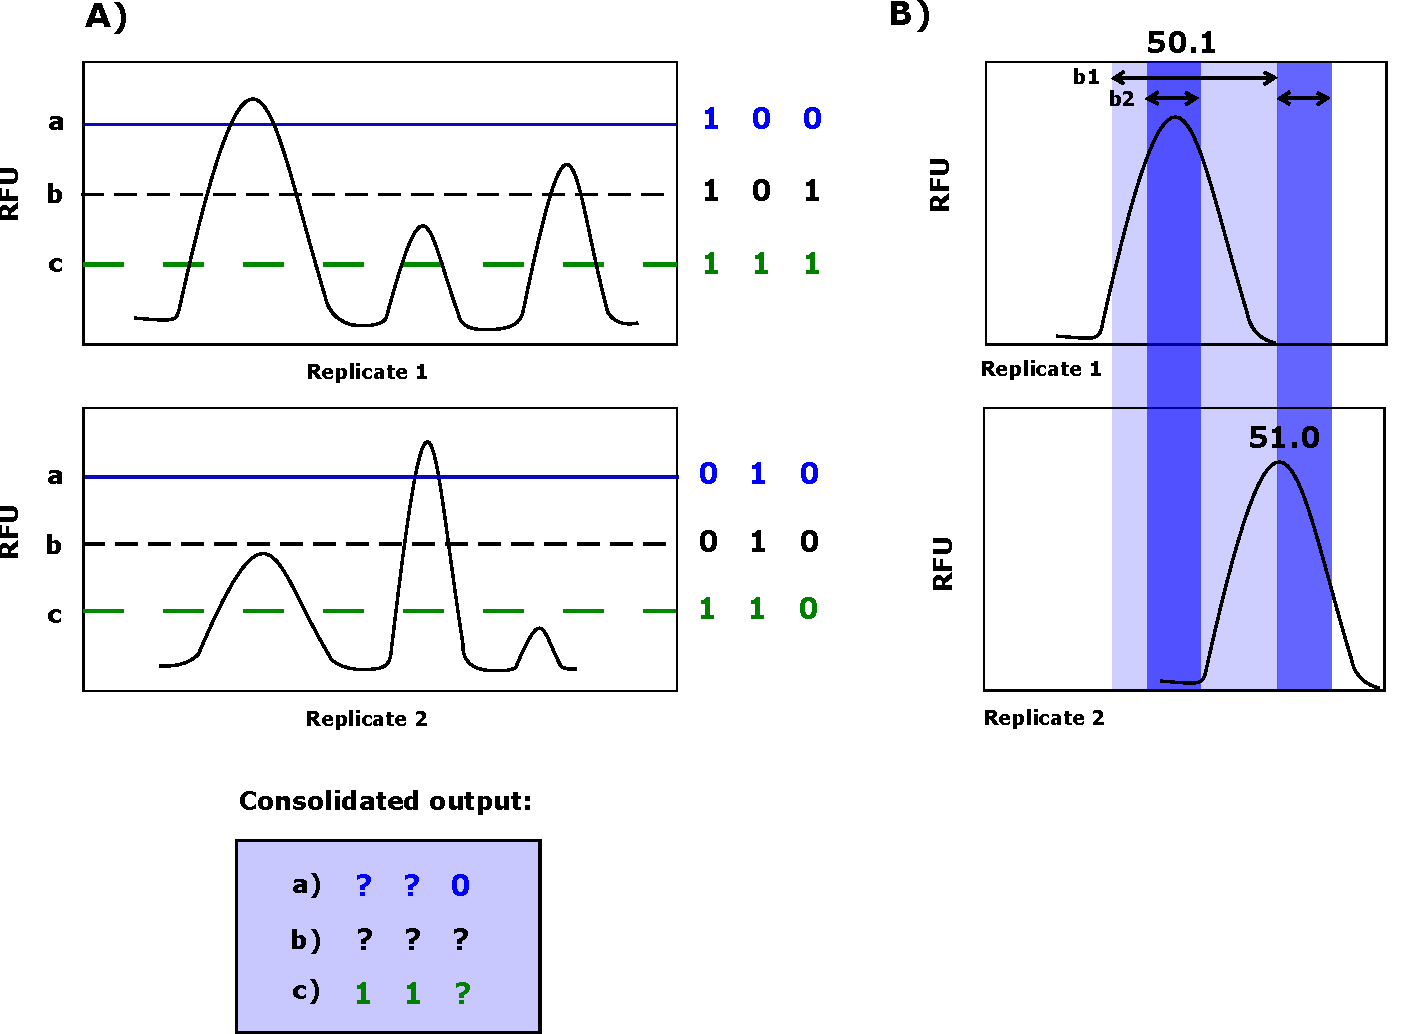
\includegraphics[scale = 0.7]{Images/source_of_scoring_errors.pdf}
	\caption{Potential sources of scoring errors in band-based genotyping methods: A) Determining the optimal threshold value to apply when scoring the presence or absence of a peak. The illustration shows three RFU (Relative Fluorescence Units) threshold levels (a, b and c), the resulting binary output at each, and the consolidated binary output representing a replicate pair (where a 1 and 0 or 0 and 1 outputs a `?', the shared presence of a band outputs a `1' and the shared absence a `0'). B) The effect of bin width on the scoring of peaks. Replicate 1 shows a band of 50.1 base pairs (bp) in size, and replicate 2 shows one of 0.9 bp larger. With a bin width set at b1, both will be scored as present at the same locus, but at a width of b2, these bands will be scored as two seperate loci.}
	\label{fig:scoring_errors}
\end{figure} 